\documentclass[../main.tex]{subfiles}

\graphicspath{../images/}

\begin{document}

\section{Vector Analysis}
\barh 

\paragraph{1.1}
\begin{figure}[ht]
    \centering
    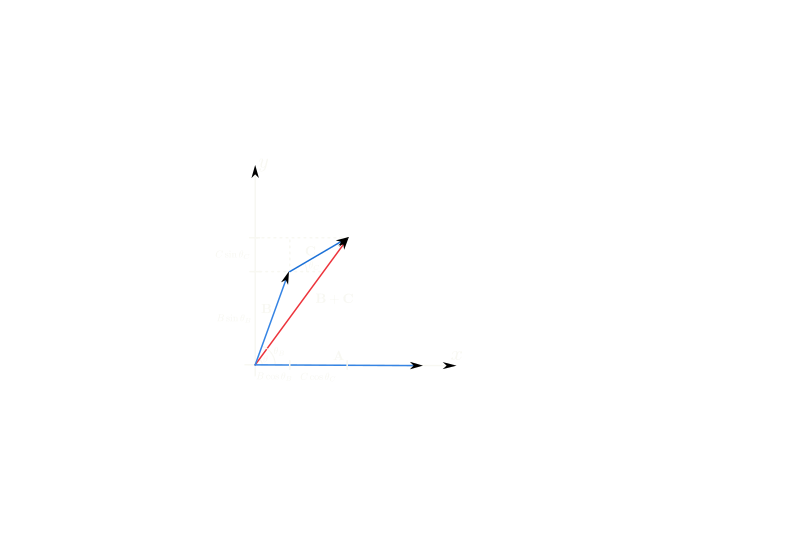
\includegraphics[width=0.5\linewidth]{images/fig1_1.png}
    \caption{Three Coplanar Vectors}
    \label{fig:1.1}
\end{figure}
(a) When three vectors are coplanar as shown in Figure \ref{fig:1.1}, the dot product is
\begin{align*}
    \vb{A} \cdot (\vb{B} + \vb{C}) &= \vb{A} \cdot \vb{B} + \vb{A} \cdot \vb{C} \\
    A (B+C) \cos \theta &= A B \cos \theta_B + A C \cos \theta_C
\end{align*}
Since $B \cos{\theta_B} + B \cos{\theta_C} = (B+C)\cos{\theta}$ from Figure \ref{fig:1.1}, the
distriubtive property holds true. The cross product also holds true since
$B \sin{\theta_B} + B \sin{\theta_C} = (B+C)\sin{\theta}$, and multiplying by $A$ on both sides
gives the same result as the distriubtive property:
\begin{align*}
    \vb{A} \cp (\vb{B} + \vb{C}) &= \vb{A} \cp\vb{B} + \vb{A} \cp\vb{C} \\
    A (B+C) \sin \theta &= A B \sin \theta_B + A C \sin \theta_C
\end{align*}

(b) In the general case in three-dimensional space, each vector has three components: \\
$\vb{A} = (A_x, A_y, A_z)$. Therefore,
\begin{align*}
    \vb{A} \cdot (\vb{B} + \vb{C}) &=
        \vb{A} \cdot (B_x + C_x, B_y + C_y, B_z + C_z) \\
    &= A_x (B_x + C_x) + A_y (B_y + C_y) + A_z (B_z + C_z) \\
    &= A_x B_x + A_y B_y + A_z B_z + A_x C_x + A_y C_y + A_z C_z \\
    &= \vb{A} \cdot \vb{B} + \vb{A} \cdot \vb{C}
\end{align*}

\paragraph{1.2}
Setting $\vb{A} = \vb{B} = (1, 1, 1)$ and $\vb{C} = (1, 1, -1)$:
\begin{align*}
    (\vb{A} \cp \vb{B}) \cp \vb{C} &\overset{?}{=} \vb{A} \cp (\vb{B} \cp \vb{C})\\
    0 &\overset{?}{=} (1, 1, 1) \cp [(1, 1, 1) \cp (1, 1, -1)]\\
    0 &\overset{?}{=} (1, 1, 1) \cp (-2, 2, 0)\\
    0 &\neq (-2, -2, 4)
\end{align*}
where the cross product of parallel vectors $\vb{A} \cp \vb{B} = 0$. Therefore, the cross product is
not associative.

\paragraph{1.3}
Taking the dot product of a unit cube's body diagonals $\vb{A} = (1, 1, 1)$, $\vb{B} = (1, 1, -1)$:
\begin{align*}
    \vb{A} \cdot \vb{B} &= AB \cos{\theta} \\
    1 &= 3 \cos{\theta} \\
    \theta &= \arccos{1/3} \approx \ang{70.53}
\end{align*} 

\paragraph{1.4}
The cross product of two vectors coplanar to the shaded plane---$\vb{A} = (-1, 2, 0)$,
$\vb{B} = (-1, 0, 3)$---is parallel to the normal unit vector $\vu{n}$ of the plane:
\begin{align*}
    \vb{A} \cp \vb{B} &= \vb{C} \\
    \begin{vmatrix}
        \vu{x} & \vu{y} & \vu{z} \\
        -1 & 2 & 0 \\
        -1 & 0 & 3
    \end{vmatrix} &= (6, 3, 2) \\
\end{align*}
where $\vu{n} = \vb{C} / C$, and $C = \sqrt{6^2 + 3^2 + 2^2} = \sqrt{49} = 7$. Therefore,
\begin{align*}
    \vu{n} &= \frac{1}{7} (6, 3, 2)
\end{align*}

\paragraph{1.5}
Proving the ``BAC--CAB'' rule for three-dimensional vectors:
\begin{align*}
    \vb{A} \cp (\vb{B} \cp \vb{C}) &= \vb{A} \cp
    \begin{vmatrix}
        \vu{x} & \vu{y} & \vu{z} \\
        B_x & B_y & B_z \\
        C_x & C_y & C_z
    \end{vmatrix} \\
    &= \begin{vmatrix}
        \vu{x} & \vu{y} & \vu{z} \\
        A_x & A_y & A_z \\
        B_y C_z - B_z C_y & B_z C_x - B_x C_z & B_x C_y - B_y C_x
    \end{vmatrix}
\end{align*}
where the $x$ component is $A_y (B_x C_y - B_y C_x) - A_z (B_z C_x - B_x C_z)$. Similarly,
\begin{align*}
    \vb{B}(\vb{A} \cdot \vb{C}) - \vb{C}(\vb{A} \cdot \vb{B}) &=
        \vb{B} (A_x C_x + A_y C_y + A_z C_z) - \vb{C} (A_x B_x + A_y B_y + A_z B_z)
\end{align*}
where $x$ component simplifes to
\begin{align*}
    B_x (\cancel{A_x C_x} + A_y C_y + A_z C_z) - C_x (\cancel{A_x B_x}+ A_y B_y + A_z B_z) &=
        A_y (B_x C_y - B_y C_x) - A_z (B_z C_x - B_x C_z)
\end{align*}
the same is done for the $y$ and $z$ components. Therefore, the ``BAC--CAB'' rule holds true.

\paragraph{1.6}
\begin{align*}
    [\vb{A} \cp (\vb{B} \cp \vb{C})] + [\vb{B} \cp (\vb{C} \cp \vb{A})] 
        + [\vb{C} \cp (\vb{A} \cp \vb{B})]
    &= \cancel{\vb{B}(\vb{A} \cdot \vb{C})} - \vb{C}(\vb{A} \cdot \vb{B})
    + \vb{C}(\vb{B} \cdot \vb{A}) = 0 \\ &- \vb{A}(\vb{B} \cdot \vb{C})
    + \vb{A}(\vb{C} \cdot \vb{B}) - \cancel{\vb{B}(\vb{C} \cdot \vb{A})}\\
\end{align*}
since dot product is associative, the first and last terms cancel out, and the middle terms also
cancel out with each other.

\begin{align*}
    \vb{A} \cp (\vb{B} \cp \vb{C}) &= (\vb{A} \cp \vb{B}) \cp \vb{C} \\
    \vb{B} (\vb{A} \cdot \vb{C}) - \vb{C} (\vb{A} \cdot \vb{B}) &=
    \vb{B} (\vb{A} \cdot \vb{C}) - \vb{A} (\vb{B} \cdot \vb{C}) \\
    0 &= -\vb{C} (\vb{A} \cdot \vb{B}) + \vb{A} (\vb{B} \cdot \vb{C}) \\
    0 &= -\vb{B} (\vb{C} \cp \vb{A}) = (\vb{C} \cp \vb{A}) \cp \vb{B}
\end{align*}
For the relation to hold true, either the vectors $\vb{A}$ and $\vb{C}$  are parallel
($\vb{A} \cp \vb{A} = 0$) or $\vb{B}$ is perpendicular to both $\vb{A}$ and $\vb{C}$
($\vb{A} \cdot \vb{B} = \vb{B} \cdot \vb{C} = 0$).

\paragraph{1.7}
Finding the seperation vector $\boldscriptr$:
\begin{align*}
    \boldscriptr &= \vb{r} - \vb{r}' = (4, 6, 8) - (2, 8, 7) = (2, -2, 1) \\
    \scriptr &= \sqrt{2^2 + (-2)^2 + 1^2} = 3 \\
    \vu{\boldscriptr} &= \quantity(\frac{2}{3}, -\frac{2}{3}, \frac{1}{3})
\end{align*}

\paragraph{1.8} (a)
\begin{align*}
    \begin{split}
        \bar{A}_y \bar{B}_y + \bar{A}_z \bar{B}_z =
        (A_y \cos{\phi} &+ A_z \sin{\phi})(B_y \cos{\phi} + B_z \sin{\phi}) \\
        &+ (-A_y \sin\phi + A_z \cos\phi)(-B_y \sin\phi + B_z \cos\phi)
    \end{split} \\
    \begin{split}
        = A_y B_y \cos^2\phi + A_z B_z \sin^2\phi
        &+ \cancel{A_y B_z \sin\phi\cos\phi} + \bcancel{A_z B_y \sin\phi\cos\phi} \\
        + A_y B_y \sin^2\phi &- \cancel{A_y B_z \sin\phi\cos\phi} 
        - \bcancel{A_z B_y \sin\phi\cos\phi} + A_z B_z \cos^2\phi
    \end{split} \\
    = A_y B_y (\sin^2\phi + \cos^2\phi) &+ A_z B_z (\sin^2\phi + \cos^2\phi) \\
    \bar{A}_y \bar{B}_y + \bar{A}_z \bar{B}_z &= A_y B_y + A_z B_z
\end{align*}
(b) To preserve length $\abs{\bar{A}} = \abs{A}$. Squaring both sides and expanding gives
\begin{align*}
    \bar{A}_x^2 + \bar{A}_y^2 + \bar{A}_z^2 = A_x^2 + A_y^2 + A_z^2
\end{align*}
in summation form,
\begin{align*}
    \sum_{i=1}^3 \bar{A}_i \bar{A}_i
    = \sum_{i=1}^3 \quantity(\sum_{j=1}^3 R_{ij} A_j) \quantity(\sum_{k=1}^3 R_{ik} A_k)
    = \sum_{i=1}^3 \sum_{j=1}^3 \sum_{k=1}^3 R_{ij} R_{ik} A_j A_k
\end{align*}
For the length to be preserved, the indices $j$ and $k$ must be equal. Therefore,
\begin{align*}
    R_{ij} R_{ik} = \delta_{jk}
\end{align*}
where $\delta_{ij}$ is the Kronecker delta. Thus the length is preserved if the rotation
matrix is orthogonal, i.e.
\begin{align*}
    R_{ij} R_{ik} = (R^T)_{ji} R_{ik} = \delta_{jk} \qor R^T R = I
\end{align*}

\paragraph{1.9}
A clockwise rotation of $\ang{120}$ about an axis through the origin and point $(1, 1, 1)$ is
equivalent to changing the position of the basis vectors $\vu{x} \to \vu{z}$, $\vu{y} \to \vu{x}$,
and $\vu{z} \to \vu{y}$. Therefore, the rotation matrix is a permutation matrix:
\begin{align*}
    R = \begin{pmatrix}
        0 & 0 & 1 \\
        1 & 0 & 0 \\
        0 & 1 & 0
    \end{pmatrix}
\end{align*}

\paragraph{1.10}

\end{document}

